\section{Der LHC und das CMS-Experiment}
\label{lhccms_chapter}
Um das Standardmodell zu \"uberpr\"ufen und Hinweise auf Physik jenseits des Modells zu erhalten bedient man sich in der Teilchenphysik oft gro\ss{}er Beschleuniger. 
Der zurzeit weltweit leistungsst\"arkste Beschleuniger ist der LHC. Er befindet sich am CERN und liefert dort den vier gro\ss{}en Experimenten Teilchenkollisionen mit einer Schwerpunktsenergie von bis zu 
$\sqrt{s} = 14\,\mathrm{TeV}$. Darunter auch dem CMS Universaldetektor, dessen aufgenommene Daten, aus dem Jahr 2011, Sie in diesem Versuch analysieren. 
Im Folgenden Kapitel werden der LHC \cite{LHC}, sowie die Identifizierung von Teilchen mit dem CMS-Detektor beschrieben. Eine ausf\"uhrliche Beschreibung der Funktionsweise eines Detektors, 
sowie der Identifizierung von Teilchen ist \cite{Kleinknecht:1984jt,Grupen:PD} zu entnehmen. 

% ======================
% ++++     LHC      ++++
% ======================
\subsection{Der Large Hadron Collider}
Der LHC ist mit einem Umfang von 26,7\,km der bislang größte von Menschen gebaute Teilchenbeschleuniger. Der Tunnel, in dem Protonen zu einer Schwerpunktsenergie von bis zu 14\,TeV beschleunigt werden,
liegt in 100\,m Tiefe am CERN\footnote{Europäische Organisation für Kernforschung. Formal \textbf{C}onseil \textbf{E}uropéen pour la \textbf{R}echerche \textbf{N}ucléaire.}-Gelände und dessen Umgebung.\\
Die durch Ionisation von Wasserstoff erzeugten Protonen \cite{duoplasma} durchlaufen eine Reihe von verschiedenen Vorbeschleunigern, bevor die Protonen in zwei gegenläufige Röhren des LHC injiziert werden (Abbildung: \ref{cernkomplex}). 
Diese Vor\-be\-schleuniger\-reihe besteht aus einem Linearbeschleuniger (LINAC 2), dem Proton Synchrotron (PS) und dem Super Proton Synchrotron (SPS). Die Protonen werden am PS auf 25\,GeV und 
anschließend am SPS auf 450\,GeV beschleunigt, ehe sie in den LHC eingespeist und an vier festgelegten Punkten zur Kollision gebracht werden. Diese Kollisionspunkte sind von den folgenden Detektoren ummantelt:
\begin{itemize}
\item ALICE (A Large Ion Collider Experiment)
\item ATLAS (A Toroidal LHC Apparatus)
\item CMS (Compact Muon Solenoid)
\item LHCb (Large Hadron Collider beauty experiment)
\end{itemize}
Die Multifunktionsdetektoren ATLAS \cite{atlas} und CMS sind so konstruiert, dass eine Vielzahl von Standardmodell-Messungen und darüber hinaus Suchen nach Physik jenseits des Standardmodells möglich sind. Außerdem konnten die ATLAS- und CMS-Experimente bereits die Existenz des Higgs-Bosons nachweisen.\\
Im Gegensatz zu den Multifunktionsdetektoren sind ALICE \cite{alice} und LHCb \cite{lhcb} für speziellere Aufgaben konstruiert. So werden bei ALICE Blei-Ionen zur Kollision gebracht, um ein Quark-Gluon-Plasma zu erzeugen und zu untersuchen. Beim LHCb-Experiment wird die CP-Verletzung von B-Mesonen untersucht.
\\
Einer der großen Vorteile des LHC im Vergleich zu vorherigen Experimenten ist seine hohe Luminosität. Die Luminosität beschreibt die Anzahl der Teilchenbegegnungen pro Zeit und Fläche und ergibt sich aus
\begin{equation}
L=\frac{n_{b}N_{p}^{2}f}{A},
\end{equation}
wobei $n_{b}$ die Anzahl der B\"undel im Teilchenstrahl, $N_{p}$ die Anzahl der Protonen im B\"undel und $f$ die Umlauffrequenz der B\"undel ist. Die Gr\"o\ss{}e $A$ entspricht der effektiven Breite des Strahls in transversaler Richtung.\\
Als Designparameter f\"ur den LHC sind dabei $n_{b}=2808$ B\"undel mit $N_{p}=1,15\cdot 10^{11}$ Protonen pro B\"undel, eine Umlauffrequenz $f=11,25$\,kHz und dar\"uber hinaus eine Luminosit\"at von $L=10^{34}$cm$^{-2}$s$^{-1}$ vorgesehen. Als ein Ma\ss{} f\"ur die Gesamtzahl von Kollisionen und der damit gesammelten Gesamtdatenmenge wird die integrierte Luminosit\"at $L_{\rm{int}}=\int L dt$ eingef\"uhrt. In diesem Praktikumsversuch untersuchen Sie einen Datensatz mit einer integrierten Luminosit\"at von 50 pb$^{-1}$.
% Abbildung \ref{intlumi} zeigt die im Jahr 2012 aufgenommene integrierte Luminosit"at bei einer Schwerpunktsenergie von 8\,TeV. Der LHC lieferte 23,3\,fb$^{-1}$, wovon der CMS-Detektor 21,8\,fb$^{-1}$ aufgenommen hat \cite{lhclumi}.
\begin{figure}[t]
	\centering
	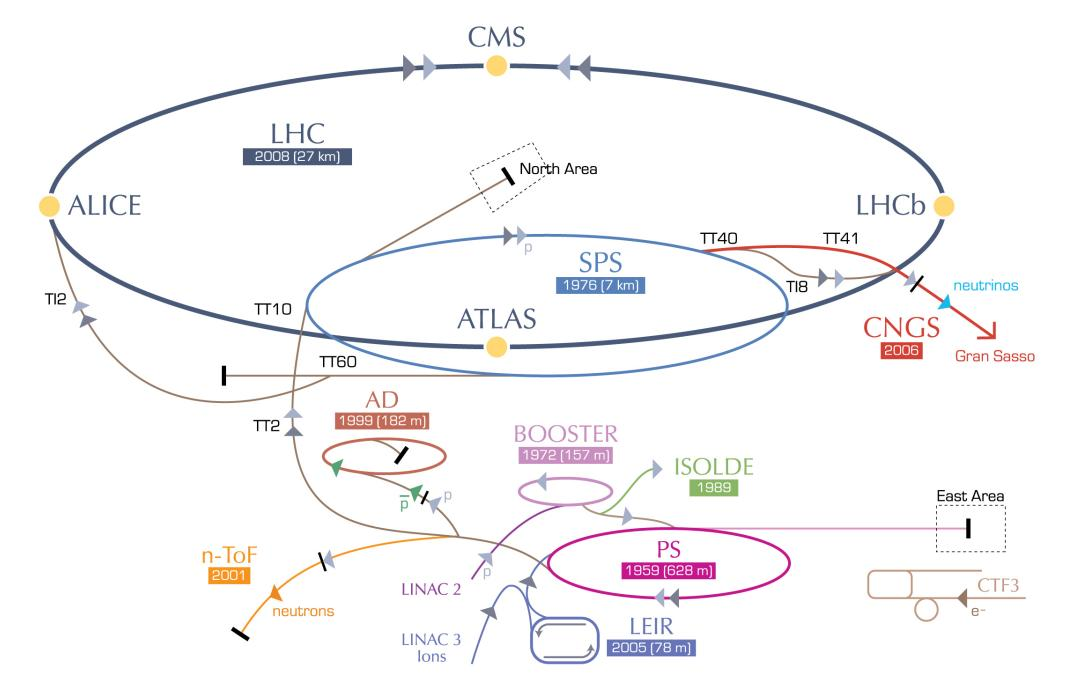
\includegraphics[scale=0.35]{LHC/CERNkomplex}
	\caption[Beschleunigerkomplex des CERN]{Beschleunigerkomplex des CERN, inklusive der vier gr\"o\ss{}ten Experimente des LHC \cite{cernkomplex}.}
	\label{cernkomplex}
\end{figure}
\subsection{Teilchen-Identifizierung im Detektor}
Bei den Kollisionen der Protonen entstehen etliche neue Teilchen, die in alle Richtungen auseinander fliegen und mit Hilfe eines Detektors vermessen werden.
In Kapitel \ref{kapsm} haben wir die Teilchen des Standard-Modells aufgelistet. Nicht alle diese Teilchen k\"onnen direkt im Detektor beobachtet werden.
So zerfallen beispielsweise die Bosonen (W, Z und Higgs) viel zu schnell, sodass lediglich die Zerfallsprodukte beobachtet und vermessen werden k\"onnen.
Identifizierbar sind z.B. Elektronen, Myonen sowie Photonen. Freie Quarks konnten bislang nicht beobachtet werden, jedoch werden sie als B\"undel von Teilchen, sogenannten Jets identifiziert.

Ein aus heutiger Sicht gew\"ohnlicher Detektor besteht aus mehreren Komponenten. Diese Komponenten sind in verschiedenen Lagen \textit{ziebelschalenf\"ormig} umeinander angeordnet.
Der CMS-Detektor ist neben dem ATLAS-Detektor einer der beiden Multifunktionsdetektoren am LHC. Ein schematischer "Uberlick des CMS-Detektors mit den meisten seiner Komponenten ist
Abbildung \ref{cmsdetektor} zu entnehmen. Die namensgebende Komponente ist der supraleitende Solenoid, welcher ein Magnetfeld von bis zu $B=4$\,T parallel zum Teilchenstrahl generiert.
Die weiteren Komponenten werden im Folgenden beschrieben.\\

	\begin{figure}[t]
		\centering
		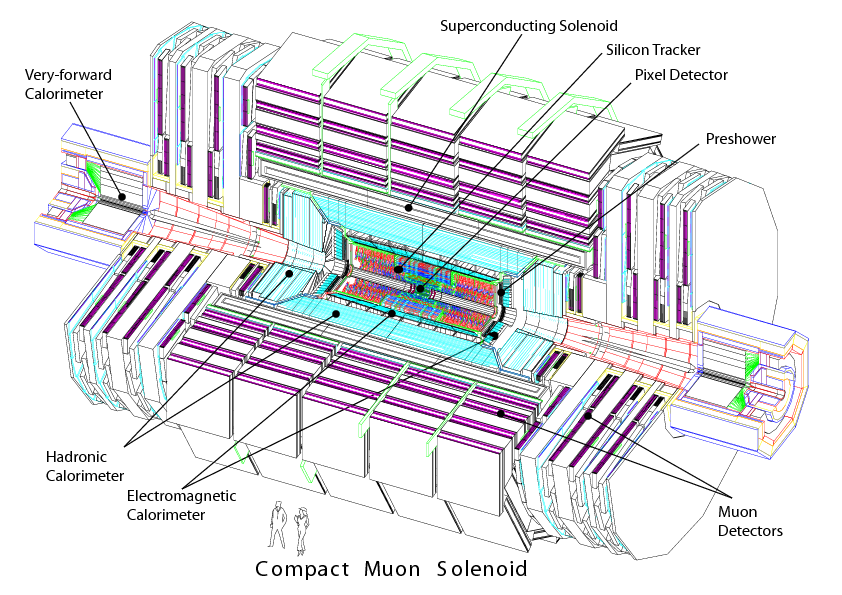
\includegraphics[scale=0.50]{LHC/cms_complete}
		\caption[Der CMS-Detektor]{Der CMS-Detektor \cite{Chatrchyan:2008aa}.}
		\label{cmsdetektor}
	\end{figure}

\begin{itemize}
\item \textbf{Spurdetektor}. Im Inneren des CMS-Detektors befinden sich sogenannte Spurdetektoren aus Silizium, die die Messung von Ladung, Richtung und Impuls von geladenen Teilchen zur Aufgabe haben. Ausserdem wird der Entstehungsort der geladenen Teilchen bestimmt. Dies ist insbesondere von Bedeutung um Mesonen zu identifizieren. Das b-Quark bzw. b-Mesonen spielen dabei eine besondere Rolle, weil sie eine vergleichsweise lange Lebensdauer haben. Diese Mesonen legen aufgrund ihrer Lebensdauer im Mittel einen Weg von einigen Millimetern zur\"uck, ehe sie in leichtere Teilchen zerfallen und k\"onnen so von anderen Mesonen unterschieden werden. 
\item \textbf{Kalorimeter}. In den Kalorimetern des CMS-Detektors wird die Energie der entstandenen Teilchen bestimmt. Beim Zusammensto{\ss} der Teilchen mit Materie entstehen neue Teilchen und Photonen, dessen Energie anschlie{\ss}end vermessen wird.\\
Unterschieden wird dabei zwischen dem elektromagnetischen und dem hadronischen Kalorimeter. Das elektromagnetische Kalorimeter (bestehend aus 80.000 Blei\-wol\-fra\-mat-Kristallen) misst die Energie von Elektronen und Photonen mit hoher Pr\"azision, indem diese Teilchen im Material einen elektromagnetischen Schauer erzeugen.\\
Das daran anschlie{\ss}ende hadronische Kalorimeter dient der Energiemessung der Hadronen, wie z.B. der Protonen oder Neutronen. Hier sind abwechselnd Lagen aus einem Material mit hoher Dichte (beim CMS-Detektor handelt es sich um Messing) als Absorbermaterial sowie Plastik-Szintillatoren als aktives Medium angebracht. 
\item \textbf{Myondetektor}. Die einzigen geladenen Teilchen, die in den Kalorimetern nicht absorbiert werden k\"onnen und diese durchdringen, sind Myonen. Zur Vermessung der Myonen ist der Magnet von sogenannten Myon-Kammern umgeben. Diese Kammern sind mit Gas gef\"ullt. Das Gas wird von den geladenen Myonen ionisiert und l\"osen so ein elektrisches Signal aus.
\end{itemize}
\begin{figure}[ht]
	\centering
	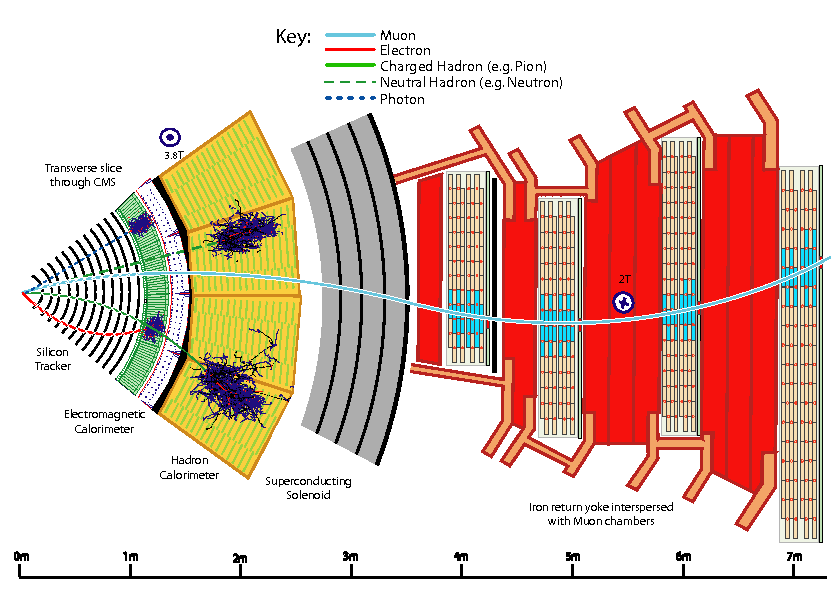
\includegraphics[scale=0.45]{LHC/cms_particle_identification}
	\caption[CMS im Querschnitt]{Querschnitt durch den CMS-Detektor. Darstellung der verschiedenen Komponenten und deren Beitrag zur Teilchenidentifikation. \cite{Sirunyan:2270046}.}
	\label{cernkomplex}
\end{figure}
\clearpage
\subsection{Jets und Jet Energie Korrekturen} 
Als Jets bezeichnet man ein B"undel von Hadronen, welches in Richtung des Ursprungs-Quarks fliegt (siehe Hadronisierung). Wie jedes experimentell rekonstruierte Objekt m\"ussen auch Jets kallibriert werden.
Die von der CMS-Gruppe bestimmten Korrekturen der Jet Energieskala ber\"ucksichtigen zusätzliche Energiebeitr\"age aus weiteren Proton-Proton Kollisionen (Pile-up), die Response des Detektors sowie
weitere Detektoreffekte. Eine detaillierte Behandlung der Korrekturen findet sich in \cite{Khachatryan:2016kdb}. Diese Jet Energie Korrekturen (JEC) sind f\"ur viele Analysen von gro\ss{}er Bedeutung und zumeist eine der wichtigsten ssystematischen Unsicherheiten.  

% xyz kann rekonstruiert werden, zyx nicht. xyz kann rekonstruiert werden in folgenden Subdetektorkomponenten. Richtung und Impuls wird aus Tracker und Magnetfeld bestimmt, Energie aus Kalorimetern
%Zyx kann aus den beobachtbaren Teilchen rekonstruiert werden -> Bedingungen bla


% +++++++++++++++++++ Spurdetektor +++++++++++++++++++++++
%\subsubsection*{Spurdetektor}
%\label{kapinnertracking}
%Zur Messung der Ladung, der Richtung und des Impulses von geladenen Teilchen ist eine pr"azise Spurrekonstruktion notwendig. Der Spurdetektor ist die innerste Komponente des CMS-Detektors und zylindrisch aufgebaut. Seine sensiblen Bauteile sind auf Silizium basierende Sensoren, welche die durch Ionisation verloren gegangene Energie geladener Teilchen messen. 
%
%
%
%\subsubsection*{Elektromagnetisches Kalorimeter}
%\label{kapemkalo}
%Das elektromagnetische Kalorimeter (ECAL) umgibt den Spurdetektor und dient zur Messung der Energie von Elektronen und Photonen, die im Material einen elektromagnetischen Schauer erzeugen. Es ist beispielsweise von wesentlicher Bedeutung zur Identifizierung eines Higgs-Bosons im Zerfallskanal $H\rightarrow \gamma\gamma$. 
%\\
%Die Leistungsf"ahigkeit des ECALs wird mit Hilfe eines Teststrahls gemessen. Die Energieaufl"osung f"ur Elektronen als Funktion der Energie kann daher wie folgt parametrisiert werden \cite{Chatrchyan:2008aa}:
%\begin{equation}
%\left(\frac{\sigma(E)}{E}\right)^{2}=\left(\frac{a}{\sqrt{E/\text{GeV}}}\right)^{2}+\left(\frac{b}{E/\text{GeV}}\right)^{2}+\left(c\right)^{2}.
%\end{equation}
%Der erste Term wird aufgrund der elektromagnetischen Schauer eingef"uhrt und ist von statistischer Natur. Der zweite Term beschreibt das Rauschen der Elektronik. Der konstante Term ist beispielsweise auf Kalibrationsfehler oder das nichtlineare Ansprechverhalten zur"uckzuf"uhren.
%
%
%
%\subsubsection*{Hadronisches Kalorimeter}
%\label{kaphadkalo}
%Das hadronische Kalorimeter (HCAL) dient der Mess\-ung der Energie von geladenen und neutralen Hadronen. Da Hadronen bei gleicher Prim"ar\-energie tiefer in Material eindringen als Photonen und geladene Leptonen, liegt das HCAL au"serhalb des ECALs und umgibt es.\\
%
%
%
%\subsubsection*{Myon-System}
%\label{kapmyonsys}
%Die am weitesten au"sen liegende Komponente des CMS-Detektors ist das Myon-System. Das Myon-System wird ben"otigt, weil Myonen als minimal ionisierende Teilchen sowohl den Spurdetektor als auch die Kalorimeter ohne auff"allige Energieverluste durchqueren. Betrachtet man den Wechselwirkungspunkt als den Ursprung der Myonen, so ist die Bestimmung des Ablenkswinkels im Myon-System essentiell f"ur eine Messung des Impulses von Myonen.\\




%\subsubsection{Trigger und Datenerfassung}
%\label{trig}
%Die Kollisionsrate der Teilchenb"undel betr"agt am LHC 40\,MHz f"ur die Designluminosit"at. Diese Rate entspricht ungef"ahr 10$^{9}$ Wechselwirkungen pro Sekunde, wovon jedes Ereignis eine Datengr"o"se von 1\,MB hat. Es k"onnen jedoch lediglich einige hundert Wechselwirkungen pro Sekunde gespeichert werden. Der Trigger hat deshalb die Aufgabe, potentiell interessante Ereignisse schnell und effizient zu selektieren. Das Trigger-System arbeitet dabei in zwei Schritten.\\
%\\
%Zun"achst wird im Level-1(L1) Trigger die Rate von weiter zu prozessierenden Ereignissen auf maximal 100\,kHz reduziert. Dieses geschieht "uber eine vereinfachte Ereignisrekonstruktion, bei der einzig die Daten aus schnellen Detektorkomponenten, wie die Kalorimeter oder das Myon-System, ausgew"ahlt werden. Die Zeit f"ur eine Entscheidung ist im L1 Trigger auf 3,2\,$\mu$s pro Ereignis beschr"ankt. M"ogliche Teilchenkandidaten werden danach "uber vereinfachte Algorithmen rekonstruiert. Letzten Endes wird ein Ereignis auf Basis von festgelegten Grenzwerten, z.B. f"ur die transversale Energie $E_{T}$ oder den transversalen Impuls $p_{T}$ von Photonen, Elektronen, Myonen oder Jets, selektiert.\\
%\\
%Im zweiten Schritt k"onnen mit Hilfe des auf Software beruhenden High-Level-Triggers (HLT) Informationen aus allen Komponenten des Detektors mit h"oher entwickelten Algorithmen analysiert werden. Potentiell interessante Ereignisse werden auf Basis umfangreicher Eigenschaften selektiert, sodass eine Ereignisrate von n"aherungsweise 300\,Hz erreicht wird. Die Zeit f"ur eine Entscheidung des HLTs ist dabei auf 50\,ms pro Ereignis beschr"ankt.
%\\
%Um die finale Ereignisrate trotz ansteigender Luminosit"at auf dem Designwert zu halten, sind unterschiedliche Methoden m"oglich. Optimal w"aren verbesserte Algorithmen, die den Untergrund st"arker unterdr"uckt. Anderenfalls k"onnen die Trigger Grenzen erh"oht werden, wodurch jedoch die Effizienz des Signals verloren gehen kann. Des Weiteren be\-steht die M"oglichkeit eine zu hohe Triggerrate mit festgelegten Grenzen aufrecht zu erhalten, indem Ereignisse mit einem \textit{prescale} $n$ aufgenommen werden, sodass lediglich jedes $n$-te Ereignis erfasst wird.

